
%(BEGIN_QUESTION)
% Copyright 2007, Tony R. Kuphaldt, released under the Creative Commons Attribution License (v 1.0)
% This means you may do almost anything with this work of mine, so long as you give me proper credit

Shielded cables are necessary for protecting small electrical signals from external interference in the form of electric fields, but one must be careful how to connect the shield wire.  Examine the following illustration, and determine which of the three installations is wired incorrectly, and why:

$$\includegraphics[width=15.5cm]{i02226x01.eps}$$

Of the two remaining installations, which of them do you think would be preferred over the other, and why?

\vskip 20pt \vbox{\hrule \hbox{\strut \vrule{} {\bf Suggestions for Socratic discussion} \vrule} \hrule}

\begin{itemize}
\item{} A principle to bear in mind here is that the earth is not a perfect conductor of electricity, and as such it is possible to develop significant voltage drops between different locations on the earth.  Propose at least one mechanism by which such a voltage drop might develop between different locations on the earth.  The fact that the earth is not a perfect conductor is not sufficient in itself to guarantee a voltage will exist between different locations -- rather, it merely {\it permits} such a phenomenon -- so there must be something else at work to actually generate the potential differences.  What might this ``something else'' be?
\end{itemize}

\underbar{file i02226}
%(END_QUESTION)





%(BEGIN_ANSWER)

The best installation is the one without a {\it ground loop}.

\vskip 10pt

When choosing between the other two shield-grounding strategies, it is best to imagine an installation where many shielded cables terminate at a single enclosure on one end, and terminate at far-flung field locations at the other ends.  What we must try to avoid here is the possibility of electric shock hazard to any technicians working on these cables, resulting from large differences in earth ground potential at different locations.

%(END_ANSWER)





%(BEGIN_NOTES)

The middle installation, with the shield wire connected to ground at both ends is incorrect.  This forms a ground loop as such:

$$\includegraphics[width=15.5cm]{i02226x02.eps}$$

The existence of a ground loop permits the formation of an electric current through the shield wire.  This, in turn, creates a magnetic field in close proximity to the signal wires which can induce a  significant amount of common-mode noise.  This may be problematic even in differential signaling systems if the induced common-mode voltage is excessive.

\vskip 10pt

Of the two remaining (acceptable) installations, the one with the cable shield grounded at the panel is generally preferred, if for no other reason than it allows for quick and easy inspection of shield ground connections at one physical location.  Grounding at a common point also eliminates the possibility of different cables having shield wires at different potentials inside the panel, which could pose a safety hazard to technicians working in the panel in certain industrial applications where ground current leakage from high-power devices may cause significant variations in earth ground potential at different sites around the facility.

%INDEX% Electronics review: ground loop, in shielded cable

%(END_NOTES)


